\begin{abstract}
Provide a short description of the project (problem studied, contributions, findings).
\end{abstract}

\section{Introduction}

A common way of organizing information on websites it to rely on tags provided
by users. Although these words are chosen freely, we do not expect them to be
arbitrary and thus hope to be able to extract limited semantics from them. In
this project, we focus on tags associated with geolocated photos extracted
from
Flickr\footnote{\href{https://secure.flickr.com/}{http://www.flickr.com/}}.
Using this crowdsourced set of (tags, location) pairs, we investigate three
problems:
\begin{itemize}
	\item Given a tag, find the places in a city where it is significantly
		concentrated.
	\item Conversely, given a location, find the tags that best describe it
		compared with other locations of similar scale.
	\item Finally, find the places in the city that seems to generate the
		most interest.
\end{itemize}

In the first case, it could be applied in a touristic context. When arriving in a
new city, a person interested in \textsf{baseball} or \textsf{streetart} could
find relevant places according to the experience of inhabitants and previous
visitors. The second answer could be used by Flickr to suggest relevant tags
when users upload photos. Consequently, more sensibly tagged photos allow more
relevant search result and improve the website user experience. The last could
for instance the first step of an automatic travel guide that select point of
interest in a city or a region.

Other applications may include inferring missing information (like location or
time of the day) from the tags or…

What are the contributions of this project?

\section{Setting}
\paragraph{Uncertainty of the data}
\begin{itemize}
	\item User id are subject to caution since nothing prevent people to
 upload photos on behalf of others. It would require serious effort to
 detect it but one may expect it is rather uncommon. Moreover, the mere
 fact that the upload take place still denotes a relation between the
 user and the photos.
	\item While timestamp issued by mobile phones are likely to be correct,
 as their internal clock is synchronized by internet, this may not
 always be the case for dedicated cameras. More concerning than usual
 drift of low quality clock is the situation of tourists coming from
 different timezone. Yet as I could not think of any simple solution to
 that problem, I just ignored it and carried on.
	\item To ensure the quality of the localization, I restrict myself to
 photos whose precision is deemed \enquote{street level} by Flickr. The
 potential problem is that it would again cost an extra request to know
 whether this location was given by GPS (in which case the camera
 position is accurate) or by the user at upload time. In the latter
 case, in addition to the general imprecision of the method, it is
 ambiguous whether this location refer the place where the photo was
 shot or the position of the photo's subject\footnote{Think of a bridge
 taken from a nearby hill.}.
	\item Finally, without additional request, the tags obtained are those
 normalized by Flickr. This normalization is not bijective but it is
 assumed that two tags with the same normalized form were close in the
 first place.
\end{itemize}

Overall, these restrictions are not really problematic. Yet there is another
one that is not specific to a given field. Users have the possibility to
upload photos by batch and assign them common location and tags. In some case,
this could skew the corresponding distributions. Take the tag
\textsf{14thstreet} as an example. One user have uploaded more than
\numprint{3500} photos at one corner street during a marathon whereas only a
handful of others users have employed this tag, which is therefore not as
popular as the raw number would suggest. To alleviate this situation, I
performed a simple preprocessing step that I will describe later.

First, I duplicated the \enquote{tags} field of every photos. Then, for each
user $u$ and each tag $t$, I computed the distribution of photos tagged $t$ by
$u$ and removed the tags from the photos that appeared more than $T=120$ times
in the same place (the same cell of the $200\time 200$ discrete grid) in the same
time (2 weeks interval). With such threshold, it removed around 20\% of all
tags and it somewhat modified the list of top tag but with no clear pattern.
But tags with very low entropy like \textsf{14thstreet} did not appeared
anymore because they lost most of their support. A better way to deal with
that issue could be to weight tags by the number of their users but it would
computationally more expensive.


\subsection{Statistical exploration}
\begin{figure}[hbtp]
\includegraphics[width=\columnwidth]{distag}
\caption{Tag distribution log-log scale over three regions of different scale.\label{f:tags}}
\end{figure}

The first thing was to look at the tags to get a sense of them. In San
Francisco after the preprocessing, there was a total of \numprint{4977625}
occurrences of the \numprint{145242} unique tags. But their distribution varies
widely, between the most popular one, \textsf{sanfrancisco}, used
\numprint{373427} times and the \numprint{101361} that are used less than 5
times. Some of them are shown in Table~\vref{tab:tags} but a more synthetic
visualization is presented in Figure~\vref{f:tags}, where we can see that like
words in a written documents, tags follows a power law.

\begin{table}[ht]
	\centering
	\begin{tabular}{lll}
		\toprule
		First 15 tags 	 & between 100 and 1000 & after \numprint{90000} \\
		\midrule
		sanfrancisco 	 & 2013 							   & sfgiantsfan \\
		california       & pacific                             & rolexbigboatseries \\
		iphoneography    & february                            & proshowgold \\
		square           & foundinsf                           & neutraface \\
		% squareformat     & dolorespark                         & natur€ \\
		instagramapp     & japaneseteagarden                   & lusty \\
		unitedstates     & boat                                & lightousetender \\
		sf               & 5k                                  & jennyholzer \\
		usa              & national                            & img0562jpg \\
		% ca               & σανφρανσίσκο                        & djguyruben \\
		san              & cruise                              & cutebaby \\
		francisco        & above                               & cardamine \\
		goldengatepark   & july2009                            & californiaproduce \\
		2010             & effortlesslyuploadedbymyeyeficard   & aroundwithb1 \\
		iphone           & dayofdecision                       & aquateenhungerforcemooninite \\
		\bottomrule
	\end{tabular}
	\caption{A sample of San Francisco tags, depending of their rank.\label{tab:tags}}
\end{table}

After making these observations, I decided to consider only tags with enough
support, both to ease the computational effort and to avoid outliers. For each
tags, I compute three simple metrics, total count, distinct users count and
time span. Using the three threshold (150 photos, 25 users, 500 days), I kept
only \numprint{1874} tags. It may seem quite restrictive but they still cover
68.6\% of all occurrences and we can always change these thresholds
later\footnote{For instance, with $(20, 2, 0)$, we get \numprint{12959} tags
and 84.4\% coverage.}.

We can then conduct a similar analysis over the locations in which photos
appear. Because of their large number, it was not convenient nor readable to
display them individually. Therefore, I discretized space as a regular grid of
size 200 by 200. In that case, each rectangular cell is around $80\times 70$
meters and I used this same method for all other spatial computation. A
natural way of visualizing them is to draw a heatmap (Figure~\vref{f:heat}).
We notice again that they are far from being uniformly distributed and that
some neighborhood are more popular than others. More quantitatively, number of
photos of each location as a function of their rank (Figure~\vref{f:pdis}), we
notice that it first follows a power law and after some point, a more
abrupt one. Moreover, the same phenomena occurs for other grid size, albeit
with different $\alpha$ coefficient. Despite this similar behavior, it was
more tricky to explicitly exclude parts of the city.

\begin{figure}[hbtp]
\includegraphics[width=\columnwidth]{../heatmap.png}
\caption{Photos count in logarithmic scale (the darker, the more
photos).\label{f:heat}}
\end{figure}

\begin{figure}[hbtp]
\includegraphics[width=\columnwidth]{../prez/pdistrib.png}
\caption{Spatial distribution of photos over three grids with different
granularity.\label{f:pdis}}
\end{figure}

Let us return to one of our original problem, find which tags describe a given
location. The first approach would to filter this \numprint{1874} tags to keep
only those that are enough concentrated at one position and reject those that
too uniformily distributed. After that, it would simply a matter of returning
those that appear in the place of interest. An example of this two kind of
tags are \textsf{museum} and \textsf{street}. As shown in Figure~\vref{f:sm},
\textsf{museum} photos are mostly located around five or six points whereas
\textsf{street} is more diffuse. But instead of looking at a map, we want a
numerical statistic that allow us to distinguish between this two cases.

\begin{figure}[hbtp]
\includegraphics[width=\columnwidth]{../prez/sm.png}
\caption{Red dots denote photos tagged \textsf{museum} while blue ones are
	\textsf{street}.\label{f:sm}}
\end{figure}

\clearpage

\section{Methods}
\begin{wrapfigure}[6]{r}{0.25\textwidth}
\centering
\vspace{-.6\baselineskip}
\begin{tikzpicture}

\node[cell] (c1) at (0cm,0cm) {$1$}; \node[cell] (c2) at (19pt,0cm) {$2$}; \node[cell] (c3) at ([xshift=19pt]c2) {$3$}; \node[cell] (c4) at ([xshift=19pt]c3) {}; \node[cell] (c5) at ([xshift=19pt]c4) {}; \node[cell] (c6) at ([xshift=19pt]c5) {$g$};

\node[cell] (c21) at ([yshift=19pt]c1) {$g+1$}; \node[cell] (c22) at ([xshift=19pt]c21) {}; \node[cell] (c23) at ([xshift=19pt]c22) {}; \node[cell] (c24) at ([xshift=19pt]c23) {}; \node[cell] (c25) at ([xshift=19pt]c24) {}; \node[cell] (c26) at ([xshift=19pt]c25) {};

\node[cell] (c31) at ([yshift=19pt]c21) {}; \node[cell] (c32) at ([xshift=19pt]c31) {}; \node[cell] (c33) at ([xshift=19pt]c32) {}; \node[cell] (c34) at ([xshift=19pt]c33) {}; \node[cell] (c35) at ([xshift=19pt]c34) {}; \node[cell] (c36) at ([xshift=19pt]c35) {};

\node[cell] (c41) at ([yshift=19pt]c31) {}; \node[cell] (c42) at ([xshift=19pt]c41) {}; \node[cell] (c43) at ([xshift=19pt]c42) {}; \node[cell] (c44) at ([xshift=19pt]c43) {}; \node[cell] (c45) at ([xshift=19pt]c44) {}; \node[cell] (c46) at ([xshift=19pt]c45) {};

\node[cell] (c51) at ([yshift=19pt]c41) {}; \node[cell] (c52) at ([xshift=19pt]c51) {}; \node[cell] (c53) at ([xshift=19pt]c52) {}; \node[cell] (c54) at ([xshift=19pt]c53) {}; \node[cell] (c55) at ([xshift=19pt]c54) {}; \node[cell] (c56) at ([xshift=19pt]c55) {};

\node[cell] (c61) at ([yshift=19pt]c51) {}; \node[cell] (c62) at ([xshift=19pt]c61) {}; \node[cell] (c63) at ([xshift=19pt]c62) {}; \node[cell] (c64) at ([xshift=19pt]c63) {}; \node[cell] (c65) at ([xshift=19pt]c64) {}; \node[cell] (c66) at ([xshift=19pt]c65) {$g^2$};
\end{tikzpicture}

% 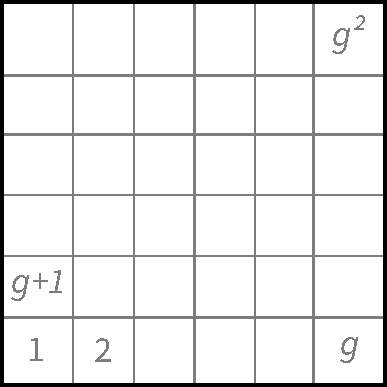
\includegraphics[width=0.15\columnwidth]{grid}
\end{wrapfigure}
Let first define some notation. As mentioned before, the city is divided in a
$g\times g$ grid made of rectangular cells $1$ through $g^2$ (like pictured on
the right). For a cell $i$, let $b(i)$ be the total number of photos in
$i$\fup{th} cell \footnote{The so called background, hence the notation.},
$B=\sum_i b(i)$ the total number of photos and $b_f(i)=\frac{b(i)}{B}$ the
frequency of each cell. For a tag $t$, we define in the same manner $t(i)$,
$T$ and $t_f(i)$, this time considering only photos which have tags $t$.

With these frequencies we can compute entropy. Let \[H(t,g) = -\frac{1}{2\log
g}\sum_{i=1}^{g^2} t_f(i)\log t_f(i)\] be the entropy of tag $t$ on a grid of
size $g$. The normalization factor ensures that regardless of $g$, the values
will range from $0$ (all photos in the same cell) to $1$ (uniform
distribution). Tags with extremal values are presented in
Table~\vref{tab:entropy} for three grids: $200\times 200$ (each cell is $80$
by $70$ meters long, less than a block), $80\times 80$ ($200\times 180$
meters, slightly more that a block) and $20\times 20$ ($800\times 700$ meters,
maybe a district). We notice that the lowest values relate to specific
location like museum while highest one are generic. Whereas $g=200$ and
$g=80$ yield comparable result, it is no more the case for $g=20$. In
particular high valued tags become even more generic (sky, dog, \dots).

\begin{table}[ht]
\centering
\setlength{\tabcolsep}{0.8em}
\begin{tabular}{lclclc}
\toprule
 \multicolumn{2}{c}{$g=200$}&  \multicolumn{2}{c}{$g=80$}&  \multicolumn{2}{c}{$g=20$}  \\
\midrule
\multicolumn{6}{c}{Lowest entropy} \\
\midrule
111minna         & .046 & theindependent         & .008 & museumofmodernart   & .002 \\
billgraham[…]    & .052 & dnalounge              & .012 & yerbabuena[…]       & .003 \\
rodin            & .053 & franklloydwright       & .022 & californiapalace[…] & .003 \\
teagarden        & .058 & greatamerican[…]       & .022 & museemecanique      & .006 \\
dnalounge        & .063 & californiapalace[…]    & .025 & cupidsspan          & .007 \\
bottomofthehill  & .064 & bottomofthehill        & .025 & pier45              & .007 \\
cafedunord       & .067 & saintspeter[…]         & .026 & missiondolorespark  & .008 \\
theindependent   & .069 & rodin                  & .034 & theindependent      & .010 \\
franklloydwright & .070 & honor                  & .035 & clarionalley        & .011 \\
warfield         & .074 & billgraham[…]          & .035 & asianartmuseum      & .012 \\
greatamerican[…] & .075 & asianartmuseum         & .038 & fairmont            & .012 \\
\midrule
\multicolumn{6}{c}{Highest entropy} \\
\midrule
usa              & .688 & color                  & .728 & sunset              & .751 \\
sf               & .696 & northerncalifornia     & .729 & dog                 & .753 \\
instagramapp     & .700 & square                 & .735 & purple              & .755 \\
square           & .700 & instagramapp           & .736 & nikon               & .756 \\
squareformat     & .700 & squareformat           & .736 & sky                 & .757 \\
iphoneography    & .703 & iphoneography          & .737 & blue                & .766 \\
unitedstates     & .703 & iphone                 & .737 & d200                & .767 \\
iphone           & .720 & california             & .738 & color               & .769 \\
foundinsf        & .724 & sanfrancisco           & .744 & northerncalifornia  & .773 \\
california       & .726 & gwsf                   & .766 & gwsf                & .812 \\
sanfrancisco     & .738 & foundinsf              & .803 & foundinsf           & .825 \\
\bottomrule
\end{tabular}
\caption{The tags with lowest and highest entropy for three different grid
	size (the abbreviated ones are \textsf{billgrahamcivicauditorium},
	\textsf{californiapalaceofthelegionofhonor},
	\textsf{yerbabuenacenterforthearts}, \textsf{greatamericanmusichall} and
\textsf{saintspeterandpaulchurch}).\label{tab:entropy}}
\end{table}

To further differentiate tags that are highly concentrated, we can compute the
Kullback Leibler divergence of their distribution with the one of all the
photos. For that, we define \[D_g(t||b) = \frac{-1}{\log
	\min_{b_f(i)>0}b_f(i)}\sum_{i=1,\, b_f(i)>0}^{g^2} t_f(i)\log
\frac{t_f(i)}{b_f(i)}\] This time, values range from $1$ (when all the $t$
photos are in the cell where there are the fewest total photos and thus are
maximally distinct) to $0$ (for $t=b$, which is not possible). Again extremal
values are shown in Table~\vref{tab:kl}. It also differentiates between the
two kinds of tag but compared with entropy, it seems more robust to change in
the grid dimensions as the three rows shows roughly the same set of tags.
Weirdly enough, there is also a semantic shift for position specific tags.
Whereas those picked by entropy were mostly buildings, here they relate more to
recreational areas like parks.

\begin{table}[ht]
\centering
\setlength{\tabcolsep}{1.2em}
\begin{tabular}{lclclc}
\toprule
 \multicolumn{2}{c}{$g=200$}&  \multicolumn{2}{c}{$g=80$}&  \multicolumn{2}{c}{$g=20$}  \\
\midrule
\multicolumn{6}{c}{Highest divergence} \\
\midrule
lakemerced     & .587 & lakemerced      & .568 & grandviewpark   & .506 \\
grandviewpark  & .563 & grandviewpark   & .554 & lakemerced      & .485 \\
hunterspoint   & .533 & hunterspoint    & .520 & sterngrove      & .484 \\
sterngrove     & .532 & westportal      & .514 & hunterspoint    & .477 \\
westportal     & .528 & sterngrove      & .512 & fortfunston     & .459 \\
catamaran      & .524 & chinabeach      & .502 & chinabeach      & .450 \\
dubocepark     & .519 & dubocepark      & .484 & westportal      & .446 \\
buenavistapark & .518 & glenpark        & .482 & nfl             & .441 \\
chinabeach     & .518 & buenavistapark  & .477 & candlestickpark & .440 \\
ccsf           & .517 & candlestickpark & .477 & glenpark        & .432 \\
glenpark       & .508 & fortfunston     & .471 & sfsu            & .430 \\
\midrule
\multicolumn{6}{c}{Lowest divergence} \\
\midrule
san           & .058 & san           & .032 & squareformat  & .011 \\
ca            & .058 & ca            & .030 & 2011          & .011 \\
instagramapp  & .055 & instagramapp  & .030 & square        & .011 \\
squareformat  & .055 & squareformat  & .030 & iphoneography & .011 \\
square        & .054 & unitedstates  & .030 & francisco     & .010 \\
iphoneography & .053 & square        & .030 & san           & .010 \\
unitedstates  & .053 & iphoneography & .029 & unitedstates  & .009 \\
usa           & .046 & usa           & .026 & ca            & .008 \\
sf            & .042 & sf            & .021 & sf            & .006 \\
california    & .021 & california    & .011 & california    & .004 \\
sanfrancisco  & .011 & sanfrancisco  & .006 & sanfrancisco  & .002 \\
\bottomrule
\end{tabular}
\caption{The tags with lowest and highest Kullback Leibler divergence for
	three different grid size.\label{tab:kl}}
\end{table}

This two statistics are interesting but they have one major drawback, they
give a single value for each tag. While this is convenient for ranking them,
it loses all the information about their position. That why we finally use the
Kulldorf spatial scan statistic\cite{kulldorff}. Let $R_{i,w,h}$ be a
rectangular region defined by its bottom left cell $i$, its width $w$ and its
height $h$ as the following set of cells: \[R_{i,w,h} = \{i + k + lg,\,
k\in\llbracket 0,\dots, w-1\rrbracket,\, l\in\llbracket 0,\dots,
h-1\rrbracket\}\] For a given $R$, what we will now call its discrepancy with
respect to tag $t$ is
\[
	d(t, R) =
\begin{dcases}
	t_f(R)\log\frac{t_f(R)}{b_f(R)} + (1-t_f(R))\log\frac{1-t_f(R)}{1-b_f(R)}
	& \text{if } \frac{t_f}{b_f} \geq \frac{1-t_f}{1-b_f} \text{ and } t_f \geq T\\
	0 & \text{otherwise}
\end{dcases}
\]
and we recognize the Kullback Leibler divergence restricted to $R$ and its
complementary. $T$ is a threshold ensuring that we consider only region with
enough support to be significant.

To compute it, we implemented the exhaustive method described in
\citep[Algorithm 3]{Agarwal2006spatial} with two modifications. First, letting
$w$ and $h$ go from $1$ to $g$, there are $g^2\cdot g\cdot g$ possible
regions. But to speed up computations and because we did not want to get
regions covering a large portion of the city, we restricted their maximum
size. Then, instead of returning the most discrepant region, we maintained a
list of the top $K$ ones. Like before, it is informative to look at
Table~\vref{t:disc} to see which tags get high and low values (over all their
regions). This time, the values are not normalized between different grid size
hence only the relative order is meaningfull. Again tag with high discrepancy
are related with locations such as parks. On the other side, tags with low
discrepancy are more difficult to interpret because they mostly do not refer
to geographic features.

\begin{table}[ht]
\centering
\setlength{\tabcolsep}{1.2em}
\begin{tabular}{lclclc}
\toprule
 \multicolumn{2}{c}{$g=200$}&  \multicolumn{2}{c}{$g=80$}&  \multicolumn{2}{c}{$g=20$}  \\
\midrule
\multicolumn{6}{c}{Highest discrepancy} \\
\midrule
grandviewpark     & 7.493 & grandviewpark   & 7.113 & grandviewpark       & 6.521 \\
sterngrove        & 7.208 & sterngrove      & 6.338 & sterngrove          & 5.998 \\
local             & 6.881 & candlestickpark & 6.318 & fortfunston         & 5.924 \\
alcohol           & 6.666 & dubocepark      & 6.152 & candlestickpark     & 5.638 \\
dubocepark        & 6.467 & pier7           & 6.072 & bayareadisco[…]     & 5.484 \\
yoda              & 6.467 & nfl             & 6.052 & nfl                 & 5.411 \\
coronaheights     & 6.374 & fortfunston     & 5.948 & chinabeach          & 5.392 \\
performer         & 6.374 & bottomofthehill & 5.917 & glenpark            & 5.338 \\
circus            & 6.371 & slims           & 5.804 & sfsu                & 5.326 \\
candlestickpark   & 6.285 & westportal      & 5.752 & westportal          & 5.258 \\
bernalheightspark & 6.158 & bayareadisco[…] & 5.732 & californiapalace[…] & 5.225 \\
\midrule
\multicolumn{6}{c}{Lowest discrepancy} \\
\midrule
instagramapp  & 0.013 & street      & 0.062 & logo        & 0.054 \\
squareformat  & 0.013 & sign        & 0.062 & friends     & 0.053 \\
square        & 0.012 & lofi        & 0.061 & sign        & 0.053 \\
iphoneography & 0.012 & hair        & 0.059 & yellow      & 0.052 \\
sf            & 0.009 & hipstamatic & 0.059 & bayarea     & 0.051 \\
xproii        & 0.008 & food        & 0.059 & shozu       & 0.051 \\
sierra        & 0.007 & motionblur  & 0.057 & party       & 0.050 \\
california    & 0.004 & large       & 0.056 & mirror      & 0.050 \\
rise          & 0.003 & 2009        & 0.056 & hipstamatic & 0.050 \\
amaro         & 0.002 & nashville   & 0.056 & purple      & 0.049 \\
sanfrancisco  & 0.001 & bayarea     & 0.055 & truck       & 0.048 \\
\bottomrule
\end{tabular}
\caption{Tags with lowest and highest discrepancy for three different grid
size (the abbreviated ones are \textsf{bayareadiscorymuseum} and
	\textsf{californiapalaceofthelegionofhonor}).\label{t:disc}}
\end{table}


\section{Experimental Evaluation}
With this last statistic, we will now see how we can answer the three initial
questions, albeit not optimally.

\subsection{Tag positioning}

To find where a tag appears, we simply compute its discrepancy over all
regions that satisfy some size constraints and we keep track of the $K$ ones
with the highest discrepancy. When this is done, we merge some of the
overlapping regions and discard the others. Namely, we rank region by
discrepancy, start from the top one, merge it with its two highest neighbors
and remove the others ones. Then we move to next cluster until we have visited
all regions once.

While this is conceptually easy, the main drawback is the sensitivity to the
scale of the grid and even for the same grid, the choice of parameters.
Figure~\vref{f:mus} show result for \textsf{museum} and Figure~\vref{f:ggp}
for \textsf{goldengatepark}. Because they cover area of small and larger size,
we see that the appropriated grid is different. The problem is that we need to
find the correct one before starting the computations.

\newgeometry{left=0.3cm,right=0.3cm,bottom=0cm,top=0.0cm}
\begin{figure}
        \centering
        \begin{subfigure}[b]{0.38\textwidth}
                \includegraphics[width=\textwidth]{mus/museum_200_130_2000_2_5.png}
                \caption{$g=200$, $K=1000$, $T=130$, $min=2$, $max=5$}
        \end{subfigure}~
        \begin{subfigure}[b]{0.38\textwidth}
                \includegraphics[width=\textwidth]{mus/museum_80_250_2000_1_4.png}
                \caption{$g=80$, $K=1000$, $T=250$, $min=1$, $max=4$}
        \end{subfigure}~

        \begin{subfigure}[b]{0.38\textwidth}
                \includegraphics[width=\textwidth]{mus/museum_200_250_2000_2_5.png}
                \caption{$g=200$, $K=1000$, $T=250$, $min=2$, $max=5$}
        \end{subfigure}~
        \begin{subfigure}[b]{0.38\textwidth}
                \includegraphics[width=\textwidth]{mus/museum_20_350_3000_1_1.png}
                \caption{$g=20$, $K=1000$, $T=350$, $min=1$, $max=1$}
        \end{subfigure}~

        \begin{subfigure}[b]{0.38\textwidth}
                \includegraphics[width=\textwidth]{mus/museum_200_300_1000_2_2.png}
                \caption{$g=200$, $K=1000$, $T=300$, $min=2$, $max=2$}
        \end{subfigure}~
        \begin{subfigure}[b]{0.38\textwidth}
                \includegraphics[width=\textwidth]{mus/museum_20_350_3000_1_4.png}
                \caption{$g=20$, $K=1000$, $T=350$, $min=1$, $max=4$}
        \end{subfigure}
        \caption{Photos with tags \textsf{museum} are blue dots and red
rectangles represent high discrepancy regions. $g$ is the subdivision of the
grid, $K$ the maximum number of regions before merging, $T$ the minimum
number of photos in a region to be considered, and $min$ and $max$ are the
size constraints of the regions in number of cells.\label{f:mus}}
\end{figure}
\begin{figure}
        \centering
        \begin{subfigure}[b]{0.38\textwidth}
                \includegraphics[width=\textwidth]{ggp/ggp_20_250_2000_1_5.png}
                \caption{$g=20$, $K=1000$, $T=250$, $min=1$, $max=5$}
        \end{subfigure}~
        \begin{subfigure}[b]{0.38\textwidth}
                \includegraphics[width=\textwidth]{ggp/ggp_80_200_1000_1_4.png}
                \caption{$g=80$, $K=1000$, $T=200$, $min=1$, $max=4$}
        \end{subfigure}~

        \begin{subfigure}[b]{0.38\textwidth}
                \includegraphics[width=\textwidth]{ggp/ggp_20_250_2000_1_6.png}
                \caption{$g=20$, $K=1000$, $T=250$, $min=1$, $max=6$}
        \end{subfigure}~
        \begin{subfigure}[b]{0.38\textwidth}
                \includegraphics[width=\textwidth]{ggp/ggp_200_100_2000_3_7.png}
                \caption{$g=200$, $K=1000$, $T=100$, $min=3$, $max=7$}
        \end{subfigure}~

        \begin{subfigure}[b]{0.38\textwidth}
                \includegraphics[width=\textwidth]{ggp/ggp_20_250_2000_1_7.png}
                \caption{$g=20$, $K=1000$, $T=250$, $min=1$, $max=7$}
        \end{subfigure}~
        \begin{subfigure}[b]{0.38\textwidth}
                \includegraphics[width=\textwidth]{ggp/ggp_200_200_1000_1_5.png}
                \caption{$g=200$, $K=1000$, $T=200$, $min=1$, $max=5$}
        \end{subfigure}
		\caption{Same as Figure~\ref{f:mus} but for
		\textsf{goldengatepark}.\label{f:ggp}}
\end{figure}
\restoregeometry

\subsection{Location describing}

We can also use discrepancy to describe a location as follows: we perform the
merging process just presented for all supported tags. For each of them, we
will thus obtain a few regions with an associated scalar value. Given a query
region, we go through this list and return matching tags, sorted by
discrepancy. Screenshots of a working demonstration are displayed in
Figure~\vref{f:loc}. One issue they do not show is that the list of results is
sometimes very sensitive to the rectangle selected. But they exhibit the
another one; this list can be very long and it would be desirable to limit it
(for instance in Alcatraz~(\ref{f:alca}), return only tags with discrepancy
above $3$). The matching process can also be improved, maybe by scaling the
discrepancy by the overlapping area between the query and the tag regions.

\begin{figure}[b]
\centering
\vspace{-2.8\baselineskip}
\includegraphics[height=0.42\textheight]{../prez/tourist.png}
\caption{The $20$ more discrepant tags are their characteristics
location.\label{f:cover}}
\end{figure}

\subsection{Map covering}

Finally, as a proxy for finding interesting locations, we tried to pave the
map with suitable tags. More precisely, we selected the highest discrepancy
region of each tag, ranked them and return the top ones. Result is shown in
Figure~\vref{f:cover}. In its current form, the visualization quickly become
unreadable if we allow overlapping tags. But there are more fundamental
issues. Namely, because it was computed with the values from the $200\times
200$ grid and regions smaller than $4$ cells at most, it misses larger areas
like the Golden Gate Park.  Moreover, discrepancy is an arguable criterion of
interest. Even if at first look, it seems to return mostly relevant locations,
it lacks flexibility and will always yield the same result, regardless of the
user typology and its preferences.

\begin{figure}
        \centering
        \begin{subfigure}[b]{0.5\textwidth}
                \includegraphics[width=\textwidth]{czoo.png}
                \caption{San Francisco Zoo, where Google Map indeed reports
the existence of a \enquote{Penguin Island}.}
        \end{subfigure}~
        \begin{subfigure}[b]{0.5\textwidth}
                \includegraphics[width=\textwidth]{cloh.png}
                \caption{California Palace of the Legion of Honor, a museum
					with many Auguste Rodin's sculptures.}
        \end{subfigure}

        \begin{subfigure}[b]{0.5\textwidth}
                \includegraphics[width=\textwidth]{calca.png}
                \caption{Alcatraz Island, aka \enquote{The Rock}, home of an
abandoned prison.\label{f:alca}}
        \end{subfigure}
		\caption{Description of three points of interest in San Francisco.\label{f:loc}}
\end{figure}


\section{Conclusion \& Future Work}
By summarizing what we have done so far, we will be able to see what
limitations can be addressed in further work. After extracting photos metadata
from Flickr and exploring their location and their tags, we computed some
statistics about them and notably the discrepancy of the most supported tags. We
then use this information to highlight various relationships between tags and
locations. But how can these results can be improved?

The first point to look at is the data. As mentioned on page~\pageref{p:data},
they come with some noise and we expect the results to be more relevant if we
manage to clean them. Yet it remains to be seen if it is worth the extra
effort. A simpler direction would be to increase their amount. This can be
done by crawling photos from others cities, to see if the same methods produce
the same results or if working only on San Francisco have introduced some
bias. Another approach would be to use more diverse sources like instagram,
foursquare or any other social networks that allows users to share localized and
tagged tags contents.

The second limitation that arose from focusing on a single area is that we
were not confronted enough with one fundamental issue of spatial analysis, the
modifiable areal unit problem\cite{scale}, which states that statistical
measurement can be profoundly affected by the choice of the spatial partition
and its characteristics size (in our case, the grid and its cells dimension).
It is an open question whether the current approach can simply be tuned to
tackle different area like states, countries or even the whole world or if it
needs radical change and scale-invariant statistics.

A related issue is that the presented approach comes with many parameters and
threshold. That would be fine if they encode some prior knowledge but the
truth is, they were chosen empirically. Indeed, the problem is mostly
unsupervised. For instance, except for specific tag like the name of
buildings, most of them can be found in several locations. Likewise, places
can be described by many tags, maybe of various relevance but with no clear
cut. Finally, finding interesting locations is rather subjective and
depending of the chosen criteria, can yield diverse results. The rather rigid
grid division is therefore quite limited, not least because not all locations
are rectangular! It may thus be more appropriate to try some unsupervised
clustering methods, for instance based on Euclidean norm in the case of the
photos locations or draw from natural language topic modeling approaches in
the case of tags\cite{topicModel}.

Even with this lack of definitive results, it would be helpful to have a way
to evaluate them. One way could be to generate artificial data from which we
know precisely what should be found inside, but it would again require some
assumption of our part. We can also create hand picked ground truth by
manually annoying tags and locations, as in \cite{Rattenbury2009}. To cope
with ambiguity, it would be even better aggregate evaluation from several
individuals\footnote{But also more time consuming, although this may be
presented as a game, like GeoGuessr: \url{http://geoguessr.com/}.}. An easier
alternative would be to manually extract famous landmarks from existing
tourist guide and assess precision and recall of the method.

Finally, whereas photos come with four kinds of information---tags, location,
user, time---we only work with the first two and it would undoubtedly be more
interesting to use all of them. Let us try to list systematically what we can
do of it.

First, by focusing on a single one and building a profile using the rest, we
may devise a similarity measure and use it to perform clustering. In the case
of users, it may divide between wealthy and not, young and old, male or female
\cite{gender}, tourist or inhabitant or richer category like family with kids
and traveler of a package tour. As said above, tags can be grouped into common
topic\footnote{Or at first, we can look at co-occurrences.}. Lastly, although
times and locations are subset of $\mathbb{R}$ and $\mathbb{R}^2$ and as such
already have a natural metric, they carry additional semantic that we would
like to exploit. For instance, we assume that by periodicity, Sundays in 2008
and 2013 share common patterns although they are far apart in time. Likewise,
maybe locations in front of the water or that consist of park have similar
characteristics.

Then we should consider pair of concepts. The present work deals with tags
\texrel locations in both directions, thus there are $\binom{4}{2} - 1$ other
to look for: tags \texrel time, tags \texrel users, locations \texrel times,
locations \texrel users and times \texrel users. Yet all of them may not be
interesting and we need to hierarchize our priorities. 

